\documentclass[10pt,twocolumn]{extarticle}
\usepackage[a4paper,margin=1.5cm,columnsep=0.7cm]{geometry}
\usepackage{amsmath,amssymb}
\usepackage{graphicx}
\usepackage{enumitem}
\usepackage{booktabs}
\usepackage{array}
\usepackage{tabularx}
\usepackage[T1]{fontenc}

\setlength{\parindent}{0pt}
\setlength{\parskip}{4pt}
\renewcommand{\arraystretch}{1.15}

\newenvironment{qoptions}{\begin{itemize}[leftmargin=1.8em,itemsep=2pt,topsep=2pt,label={}]}{\end{itemize}}
\newcommand{\opt}[2]{\item[({#1})] {#2}}

\newcommand{\sectionhdr}[1]{\par\vspace{4pt}\noindent\textbf{\large #1}\par\vspace{2pt}}
\newcommand{\subsectionhdr}[1]{\par\vspace{3pt}\noindent\textbf{#1}\par\vspace{2pt}}

\pagestyle{empty}

\begin{document}
\twocolumn[
\begin{center}
{\LARGE\bfseries JEE (Main+Advanced) Score-II --- Test 04 (07 May 2021)}
\end{center}
\vspace{6pt}
]

\sectionhdr{PAPER-1}

\sectionhdr{PART-1: PHYSICS}
\subsectionhdr{Section-I (i): Single Correct}

\textbf{1.} A point charge Q is placed at distance `d' from centre of a hollow sphere with inner radius `a' and outer radius `b'. A point charge `q' is also placed at centre of hollow sphere. Then the interaction potential energy of sphere and point charge `q' placed at centre will be:

\begin{center}
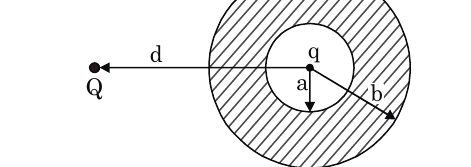
\includegraphics[width=0.65\linewidth]{Score-II - Test 04 (07 May 2021)-img/p1phy_q1_sphere.png}
\end{center}

\begin{qoptions}
\opt{A}{$kq^2\left[\dfrac1b-\dfrac1a\right]$}
\opt{B}{$kQq\left[\dfrac1b-\dfrac1a\right]$}
\opt{C}{$kQq\left[\dfrac1b-\dfrac1a+\dfrac1d\right]$}
\opt{D}{zero}
\end{qoptions}

\textbf{2.} A radioactive sample with half life $=T$ emits $\alpha$-particle. Its total activity is $A_i$ at some time and $A_f$ at a later time. The number of $\alpha$-particles emitted by the sample between these two points of time is-

\begin{qoptions}
\opt{A}{$A_i-A_f$}
\opt{B}{$\dfrac{T}{\ln2}(A_i-A_f)$}
\opt{C}{$\dfrac{\ln2}{T}[A_i-A_f]$}
\opt{D}{$\dfrac{T}{\ln2}\left[\dfrac{1}{A_i}-\dfrac{1}{A_f}\right]$}
\end{qoptions}

\textbf{3.} The circuit is completed at $t=0$, then total work done by batteries till the capacitor gets full charged. [$q_0=64\mu$C and $C=16\mu$F]

\begin{center}
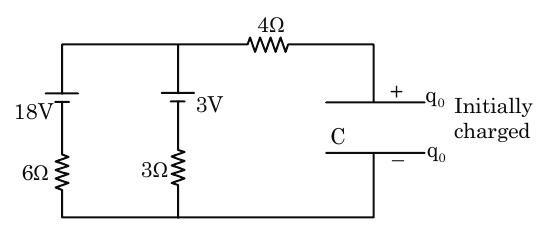
\includegraphics[width=0.75\linewidth]{Score-II - Test 04 (07 May 2021)-img/p1phy_q3_circuit.png}
\end{center}

\begin{qoptions}
\opt{A}{1024 $\mu$J}
\opt{B}{512 $\mu$J}
\opt{C}{320 $\mu$J}
\opt{D}{64 $\mu$J}
\end{qoptions}

\textbf{4.} If a string of length $\ell$ fixed at both ends vibrates with a standing wave $y=A\sin\left(\dfrac{2\pi}{\ell}x\right)\sin2\pi t$ in resonance. Then the minimum time after which energy is maximum at mid-point of string will be-

\begin{qoptions}
\opt{A}{$\dfrac14$ sec}
\opt{B}{$\dfrac15$ sec}
\opt{C}{$\dfrac18$ sec}
\opt{D}{$\dfrac16$ sec}
\end{qoptions}

\textbf{5.} Figure shows an object `O' placed in front of a equi-convex lens $\left(\mu=\dfrac32\right)$ and a plane mirror at a distance of 20 cm from lens. Point object O is placed at a distance of 45 cm from the lens. If the position of the image of the object coincides with the object itself, then radius of curvature of lens is -

\begin{center}
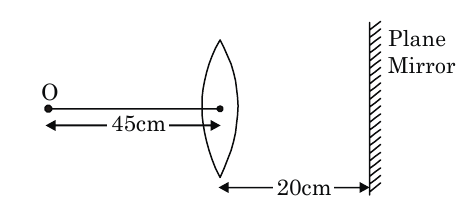
\includegraphics[width=0.65\linewidth]{Score-II - Test 04 (07 May 2021)-img/p1phy_q5_lens.png}
\end{center}

\begin{qoptions}
\opt{A}{45 cm}
\opt{B}{30 cm}
\opt{C}{60 cm}
\opt{D}{10 cm}
\end{qoptions}

\textbf{6.} Equivalent resistance between A and B will be

\begin{center}
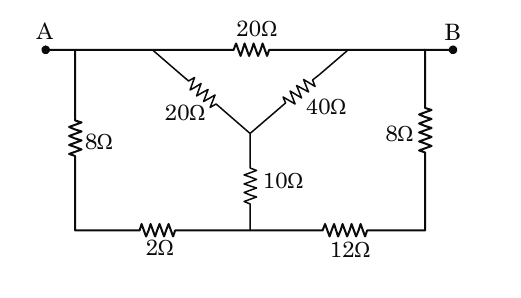
\includegraphics[width=0.75\linewidth]{Score-II - Test 04 (07 May 2021)-img/p1phy_q6_network.png}
\end{center}

\begin{qoptions}
\opt{A}{20 $\Omega$}
\opt{B}{80 $\Omega$}
\opt{C}{60 $\Omega$}
\opt{D}{10 $\Omega$}
\end{qoptions}

\textbf{7.} Two bodies A and B have the same surface area and mass. The bodies have absolute temperature $T_A$ and $T_B$, emissivities $e_A$ and $e_B$, and specific heat capacities $s_A$ and $s_B$. The intensity of radiation near a given wavelength, E, is shown plotted against the wavelength ($\lambda$) of radiation for both bodies. Which of the following is possible?

\begin{center}
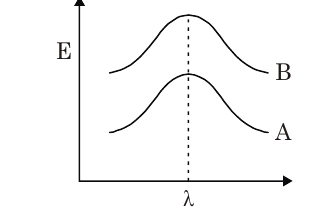
\includegraphics[width=0.42\linewidth]{Score-II - Test 04 (07 May 2021)-img/p1phy_q7_radiation.png}
\end{center}

\begin{qoptions}
\opt{A}{$T_A=T_B$, $e_A=e_B$, $S_A\ne S_B$}
\opt{B}{$T_A=T_B$, $e_A\ne e_B$, $S_A=S_B$}
\opt{C}{$T_A\ne T_B$, $e_A=e_B$, $S_A=S_B$}
\opt{D}{$T_A\ne T_B$, $e_A=e_B$, $S_A\ne S_B$}
\end{qoptions}

\textbf{8.} A larger ring of mass M and two small rings of mass `m' start rotating with angular velocity `$\omega_0$' from the position as shown in figure. Initially small rings are close to axis. There is no friction at any contact surface. Then as time passes. (Consider the motion of small rings till they move upto the bottom most point)

\begin{center}
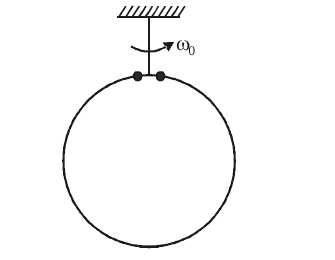
\includegraphics[width=0.4\linewidth]{Score-II - Test 04 (07 May 2021)-img/p1phy_q8_ring.png}
\end{center}

\begin{qoptions}
\opt{A}{Angular momentum of system increases.}
\opt{B}{Angular momentum of system decreases.}
\opt{C}{Angular momentum of small rings increases continuously.}
\opt{D}{Angular momentum of small rings first increases and then decreases.}
\end{qoptions}

\subsectionhdr{Section-I (ii): One or more correct (Paragraph based)}

\textit{Paragraph for Questions 9 and 10}

A fan operates at 200 V (d.c.) consuming 1000 W when running at full speed. Its internal wiring has resistance $1\Omega$. When the fan runs at full speed, its speed becomes constant. This is because the torque due to magnetic field inside the fan is balanced by the torque due to air resistance on the blades of the fan and torque due to friction between the fixed part and the shaft of the fan. The electrical power going into the fan is spent (i) in the internal resistance as heat, call it $P_1$. (ii) in doing work against internal friction and air resistance producing heat, sound, etc., call it $P_2$. When the coil of fan rotates, an e.m.f. is also induced in the coil. This opposes the external e.m.f. applied to send the current into the fan. This e.m.f. is called back e.m.f., call it e. Answer the following questions when the fan is running at full speed.

\textbf{9.} Choose the CORRECT statement(s)

\begin{qoptions}
\opt{A}{Current flowing into the fan is 5 Amp.}
\opt{B}{Current flowing into the fan is 10 Amp.}
\opt{C}{The value of back emf is 195 volt.}
\opt{D}{The value of back emf is 200 volt.}
\end{qoptions}

\textbf{10.} Choose the CORRECT statement(s)

\begin{qoptions}
\opt{A}{The value of power $P_1$ is 1000 W}
\opt{B}{The value of power $P_1$ is 25 W}
\opt{C}{The value of power $P_2$ is 900 W}
\opt{D}{The value of power $P_2$ is 975 W}
\end{qoptions}

\textit{Paragraph for Questions No. 11 and 12}

The universal gravitational constant is measured experimentally using Cavendish's experiment. This experiment is a very precise experiment which gives the value of G as $(6.6742\pm0.0010)\times10^{-11}$ N.m$^2$/kg$^2$. Since the universal gravitational constant has some error in it, using it if we find escape speed and acceleration due to gravity on Earth's surface, our values will have error in it. (Assume mass of Earth $=6.0000\times10^{24}$ kg \& radius of Earth $=6.4000\times10^6$ m.). The measurement of mass of Earth has an error of 0.01\% and radius of Earth has an error of 0.02\%.

\textbf{11.} Choose the CORRECT option(s):

\begin{qoptions}
\opt{A}{Maximum percentage error in acceleration due to gravity g $=0.065$}
\opt{B}{Maximum percentage error in acceleration due to gravity g $=0.025$}
\opt{C}{value of acceleration due to gravity g(approx. in m/s$^2$) $=9.78$}
\opt{D}{value of acceleration due to gravity g(approx. in m/s$^2$) $=8.78$}
\end{qoptions}

\textbf{12.} What will be the maximum percentage error in calculating the escape speed on earth.

\begin{qoptions}
\opt{A}{0.045\%}
\opt{B}{0.0225\%}
\opt{C}{0.015\%}
\opt{D}{0.0025\%}
\end{qoptions}

\subsectionhdr{Section-II: Numerical Value}

\textbf{1.} Two current carrying wire of infinite length are placed perpendicular to x-y plane at $x=0$ and $x=R\sqrt3$ as shown in figure. Current in both the wires is same and inwards to the x-y plane. Find ratio of $\left|\displaystyle\int\vec B\cdot d\vec\ell\right|$ in segment CDA to segment ABC will be:

\begin{center}
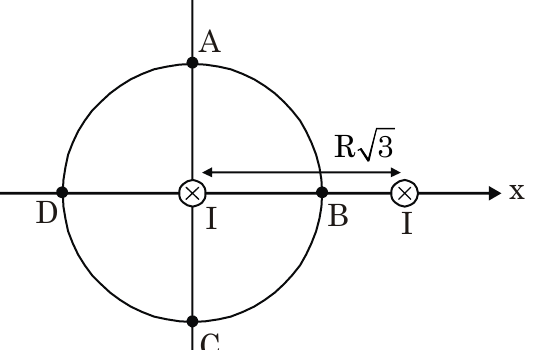
\includegraphics[width=0.55\linewidth]{Score-II - Test 04 (07 May 2021)-img/p1phy_n1_wires.png}
\end{center}

\textbf{2.} Two balls of radii r and $\dfrac r2$ are released inside a deep water tank. Their initial accelerations are found to be g/2 and g/4 respectively. If the velocity of smaller ball relative to the larger ball a long time after the two balls are released is $\dfrac{Pr^2\rho g}{\eta}$ upwards. Find P. (Coefficient of viscosity of liquid is $\eta$ and density of liquid is $\rho$).

\textbf{3.} A resistance (R), inductance (L) and capacitance (C) are connected in series to an ac source of voltage v having variable frequency. If the energy delivered by the source to the circuit during one period if the operating frequency is twice the resonance frequency is $\dfrac{\pi R\sqrt{LC}\,V^2}{R^2+P\left(\dfrac LC\right)}$ Find P.

\textbf{4.} A disc of radius R and mass M is pivoted at the rim about an axis which is perpendicular to its plane and its set for small oscillations. If the simple pendulum has to have the same period as that of the disc, then find the length (in meter) of simple pendulum if $R=\dfrac12$ m

\textbf{5.} In a searle's experiment, the diameter of the wire as measured by a screw gauge is 0.050 cm. Pitch of screw gauge is 2 mm and number of divisions on circular scale are 200. The length, measured by a scale of least count 0.1 cm is 100 cm. When a weight of 50 N is suspended from the wire elongation is measured to be 0.125 cm by a micrometer of least count 0.001 cm. Find the maximum percentage error is the measurement of young's modulus of the material of the wire from these data.

\textbf{6.} A cylinder of mass M and radius R moves with constant speed v through a region of space that contains dust particles of mass m which is at rest. There are n number of particles per unit volume. The cylinder moves in a direction perpendicular to its axis. Assume $m\ll M$, and assume the particles do not interact with each other. All the collision takes place is perfectly elastic and the surface of the cylinder is smooth. The drag force per unit length of the cylinder require to maintain the speed v constant for the cylinder when it has entered in the region is $\dfrac K3 nmRv^2$. Find the value of K.

\begin{center}
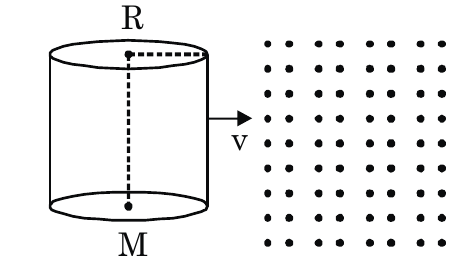
\includegraphics[width=0.42\linewidth]{Score-II - Test 04 (07 May 2021)-img/p1phy_n6_cylinder.png}
\end{center}

\textbf{7.} In a young's double slit experement, the angular separation of interference fringes on a distant screen in 0.04 \AA. The angular separation if the entire apparatus is inmerred in a liquid of refractive index $\dfrac43$ and distance between slits become half is 0.0 n\AA\ then what is the value of n?

\textbf{8.} A binary star is a system of two stars moving around the centre of inertia of the system due to mutual gravitational force. If the total mass of two stars $=M_0$ and the period of revolution is T. Find the distance in km between stars? (Take $GM_0=8\times10^6$ and $T=2\pi\times10^3$ seconds).

\sectionhdr{PART-2: CHEMISTRY}
\subsectionhdr{Section-I (i): Single Correct}

\textbf{1.} Among the given reactions, which is the best example of S$_N$2 reaction?

\begin{center}
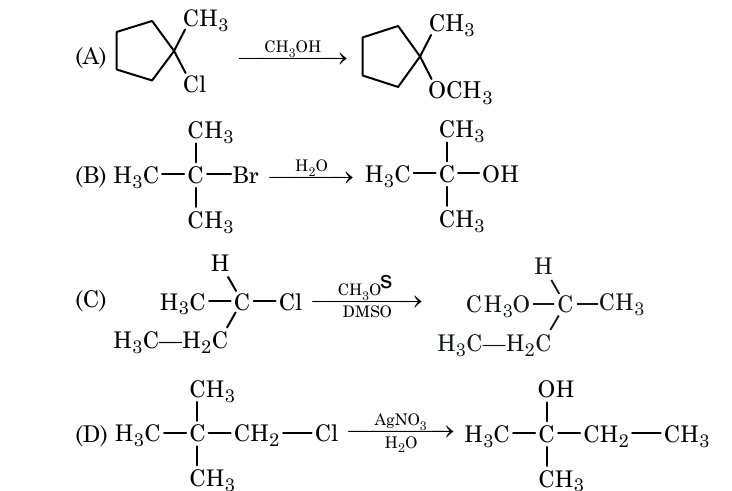
\includegraphics[width=0.95\linewidth]{Score-II - Test 04 (07 May 2021)-img/p1chem_q1_reactions.png}
\end{center}

\textbf{2.} In the given reaction, final product (X) will be;

\begin{center}
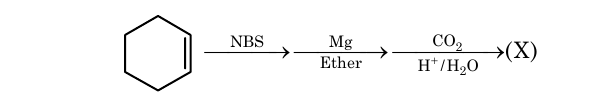
\includegraphics[width=0.55\linewidth]{Score-II - Test 04 (07 May 2021)-img/p1chem_q2_scheme.png}
\end{center}

\begin{center}
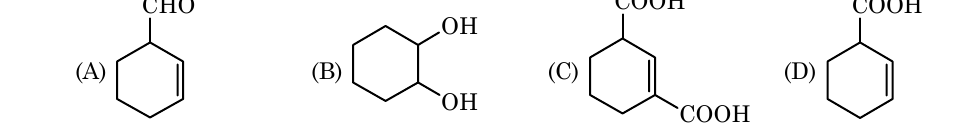
\includegraphics[width=0.95\linewidth]{Score-II - Test 04 (07 May 2021)-img/p1chem_q2_reaction.png}
\end{center}

\textbf{3.} Identify which reaction(s) produce(s) single optically active Amine molecule as product

\begin{center}
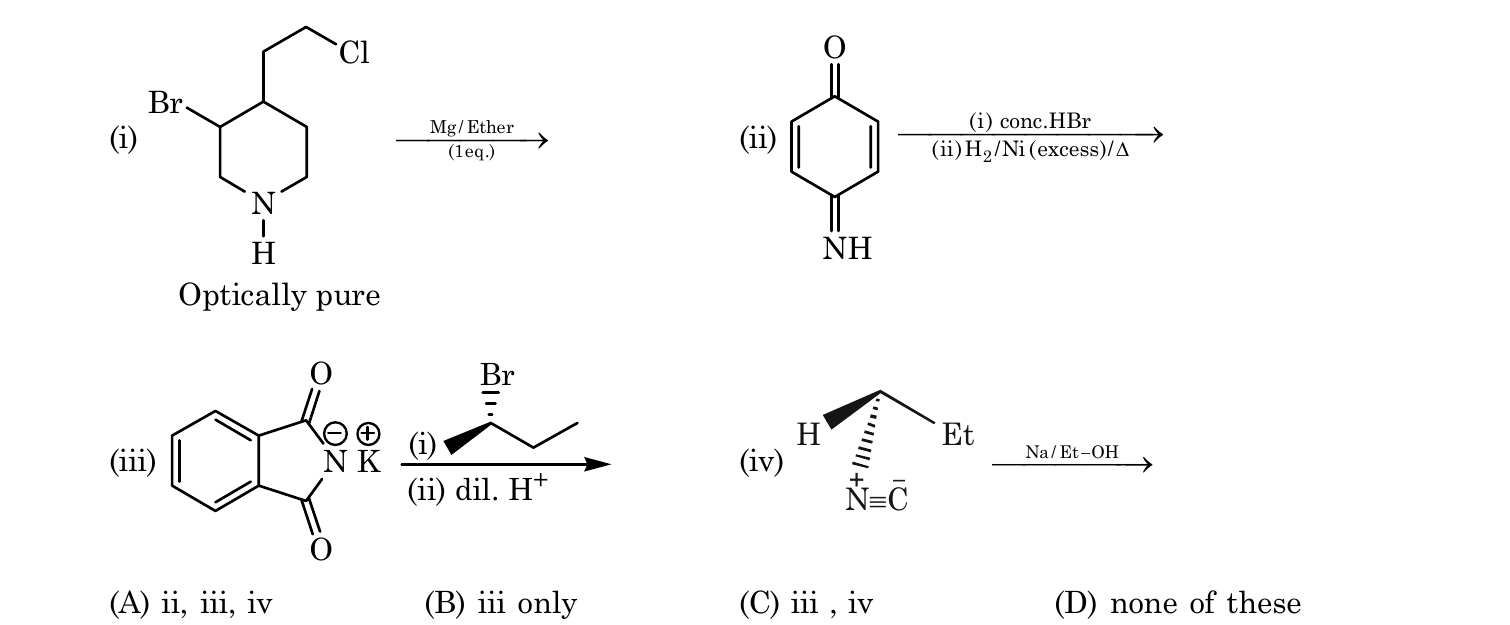
\includegraphics[width=0.95\linewidth]{Score-II - Test 04 (07 May 2021)-img/p1chem_q3_amines.png}
\end{center}

\begin{qoptions}
\opt{A}{ii, iii, iv}
\opt{B}{iii only}
\opt{C}{iii, iv}
\opt{D}{none of these}
\end{qoptions}

\textbf{4.} In an CCP crystal of metal \textbf{M} (diameter $=$ `a' \AA), we are trying to dope two smaller elements \textbf{X} (radius $=$ `0.16a' \AA) and/or \textbf{Y} (radius $=$ `0.25a' \AA) without disturbing \textbf{M-M} contact, then select correct matching.

\begin{center}
\renewcommand{\arraystretch}{1.3}
\begin{tabular}{@{}p{0.46\linewidth}p{0.46\linewidth}@{}}
\textbf{OBSERVATIONS} & \textbf{REASONS}\\
(A) Octahedral voids can have both X \& Y & O-Voids are bigger than T-voids\\
(B) Density of crystal increases on adding X & X atoms are heavier than M atoms and size of Unit cell remains same\\
(C) Packing Fraction remains same on adding X & Dimensions of unit cell remain same\\
(D) Tetrahedral Void can't have either X or Y & $\dfrac{r_X}{r_M}=0.32>$ Radius ratio of ideal Tetrahedral void\\
\end{tabular}
\renewcommand{\arraystretch}{1.15}
\end{center}

\textbf{5.} Some aqueous solutions are given below. Find the solution whose pH changes maximum by adding 10 millimoles amount of pure H$_2$SO$_4$. [$\log7=0.84$]

\begin{qoptions}
\opt{A}{100 mL, 0.1 M HCl $+$ 100 mL, 0.5 M Ca(OH)$_2$}
\opt{B}{100 mL, 0.1 M Ca(OH)$_2$ $+$ 100 mL, 0.4 M H$_2$S}
\opt{C}{100 mL, 0.1 M NaOH $+$ 100 mL, 0.2 M K$_2$SO$_4$}
\opt{D}{100 mL, 0.5 M CH$_3$COOH $+$ 100 mL, 0.1 M Ba(OH)$_2$}
\end{qoptions}

\textbf{6.} Assuming all non-hydrogenic atoms undergo hybridization \& following are various categories of orbital overlapping.
\[\text{sp}^3\text{--sp}^3 \text{ axial overlap } (\sigma) \longrightarrow \text{Type--A}\]
\[\text{sp}^2\text{--sp}^2 \text{ axial overlap } (\sigma) \longrightarrow \text{Type--B}\]
\[\text{sp}^3\text{--sp}^2 \text{ axial overlap } (\sigma) \longrightarrow \text{Type--C}\]
\[\text{p--p lateral overlap } (\pi) \longrightarrow \text{Type--D}\]
\[\text{p--d lateral overlap } (\pi) \longrightarrow \text{Type--E}\]
Identify the species which contain only 2 of these types (from A to E) of overlapping of orbitals.

\begin{qoptions}
\opt{A}{H$_2$CO$_3$}
\opt{B}{B$_3$N$_3$H$_3$F$_3$}
\opt{C}{SNF$_3$}
\opt{D}{H$_2$S$_4$O$_6$}
\end{qoptions}

\textbf{7.} Identify how many ``Ore names'', ``Type of Anion'', ``Metal(s) present in mineral'' are correctly related
\begin{center}
\renewcommand{\arraystretch}{1.15}
\begin{tabular}{@{}lll@{}}
(i) Magnetite & oxide & Fe\\
(ii) Cryolite & fluoride & Al\\
(iii) Copper Pyrite & Sulphide & Fe\\
(iv) Galena & sulphide & Hg\\
(v) Asbestos & Silicate & Al\\
(vi) Lunar Caustic & hydroxide & Ag\\
(vii) Dolomite & carbonate & Ca\\
(viii) Dolomite & hydroxide & Mg\\
\end{tabular}
\end{center}

\begin{qoptions}
\opt{A}{3}
\opt{B}{4}
\opt{C}{5}
\opt{D}{6}
\end{qoptions}

\textbf{8.} When a mixture of NaCl and K$_2$Cr$_2$O$_7$ is gently warmed with conc. H$_2$SO$_4$\\
(i) an orange-red vapour is evolved\\
(ii) the vapour formed when passed into NaOH solution gives yellow solution of Na$_2$CrO$_4$\\
(iii) Chlorine gas is not evolved at all\\
(iv) chromyl chloride gas is formed\\
(v) SnCl$_4$ used instead of NaCl also gives same observations

\begin{qoptions}
\opt{A}{All statements are correct}
\opt{B}{2 statements are correct}
\opt{C}{3 statements are correct}
\opt{D}{none of the statements are correct}
\end{qoptions}

\subsectionhdr{Section-I (ii): One or more correct (Paragraph based)}

\textit{Paragraph for Questions 9 and 10}

Monosaccharides have $-$CHO (or C$=$O) and $-$OH groups, so they undergo usual oxidation and reduction. Further, monosaccharides from osazone when treated with excess of phenylhydrazine (3 equivalents). In osazone formation only the first two carbon atoms are involved. Thus monosaccharides having identical configuration on reset of C atoms except first two will form same osazone, as is the case with glucose and fructose. A, B and C are three hexoses and form same osazone D. Compounds A to D behave as below:
\[\text{(i)}\ D\xrightarrow{\text{HCl/H}_2\text{O}}\xrightarrow{\text{Zn/CH}_3\text{COOH}}D\text{-Fructose}\]
\[\text{(ii)}\ A\xrightarrow{\text{Ni,H}_2}\xrightarrow{\text{HNO}_3}\xrightarrow{\text{Na-Hg/H}_3\text{O}^+}B+C\]
\[\text{(iii)}\ B\xrightarrow{\text{HNO}_3}\text{Optically active sacharic acid}\]
\[\text{(iv)}\ C\xrightarrow{\text{HNO}_3}\text{Optically active sacharic acid}\]

\textbf{9.} Compound A should be

\begin{qoptions}
\opt{A}{D-glucose}
\opt{B}{D-fructose}
\opt{C}{L-glucose}
\opt{D}{L-fructose}
\end{qoptions}

\textbf{10.} Compound B and C, are

\begin{qoptions}
\opt{A}{D-glucose}
\opt{B}{D-fructose}
\opt{C}{L-glucose}
\opt{D}{D-mannose}
\end{qoptions}

\textit{Paragraph for Questions 11 and 12}

The driving force $\Delta G$ diminishes to Zero on the way to equilibrium, first as in any other spontaneous process. Both $\Delta G$ and the corresponding cell potential $\left(E=\dfrac{-\Delta G}{nF}\right)$ are zero when the redox reaction comes to equilibrium. At equilibrium, the nernst equation is given as $E^0=\dfrac{0.059}{n}\log_{10}K$.

\textbf{11.} On the basis of information available for the reaction
\[\dfrac43\text{Al}+\text{O}_2\longrightarrow\dfrac23\text{Al}_2\text{O}_3,\ \Delta G=-827\text{ kJ/mole of O}_2.\]
The minimum emf required to carry out an electrolysis of Al$_2$O$_3$ is

\begin{qoptions}
\opt{A}{2.14 V}
\opt{B}{4.28 V}
\opt{C}{6.42 V}
\opt{D}{8.56 V}
\end{qoptions}

\textbf{12.} Given that, $E^o_{\text{Ni}^{2+}/\text{Ni}}=-0.25$V, $E^o_{\text{Cu}^{2+}/\text{Cu}}=+0.34$V, $E^o_{\text{Ag/Ag}^+}=-0.80$V, $E^0_{\text{Zn/Zn}^{2+}}=0.76$V

Which of the following redox process will not takes place in standard state?

\begin{qoptions}
\opt{A}{Ni$^{2+}_{(aq)}+$Cu$_{(s)}\to$ Ni$_{(s)}+$Cu$^{2+}_{(aq)}$}
\opt{B}{Cu$_{(s)}+2$Ag$^+_{(aq)}\to$Cu$^{2+}_{(aq)}+2$Ag$_{(s)}$}
\opt{C}{Ag$_{(s)}+$H$^+_{(aq)}\to$Ag$^+_{(aq)}+\dfrac12$H$_2\uparrow$}
\opt{D}{Zn$_{(s)}+2$Ag$^+_{(aq)}\to$Zn$^{2+}_{(aq)}+2$Ag$_{(s)}$}
\end{qoptions}

\subsectionhdr{Section-II: Numerical Value}

\textbf{1.} o--aminobenzaldehyde is heated along with acetone in dilute NaOH solution to produce the major organic product (A), which on treatment with catalytic amount of H$_2$SO$_4$, produces another major organic product (B) formed via intramolecular reaction. Let, the degree of unsaturation of (A) be `x'; the degree of unsaturation of (B) be `y'; the number of rings in (A) be `z' and the number of rings in (B) be `p', then, find the value of $\left(\dfrac{x.y}{z}\right)$

\textbf{2.} Given below are two reaction sequences.

\begin{center}
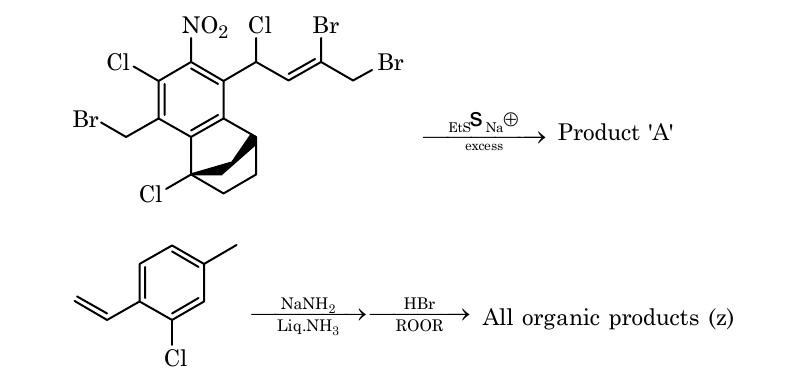
\includegraphics[width=0.85\linewidth]{Score-II - Test 04 (07 May 2021)-img/p1chem_q2_structures.png}
\end{center}

For product `A' of \textbf{REACTION-1} (no intramolecular mechanism), $x=\dfrac{\text{mass of Br atoms in 'A'}}{\text{mass of Cl atoms in 'A'}}$

For \textbf{REACTION-2}, $z=$ total no. of organic products including stereoisomers

Find value of $(x+z)=$?

\textbf{3.}

\begin{center}
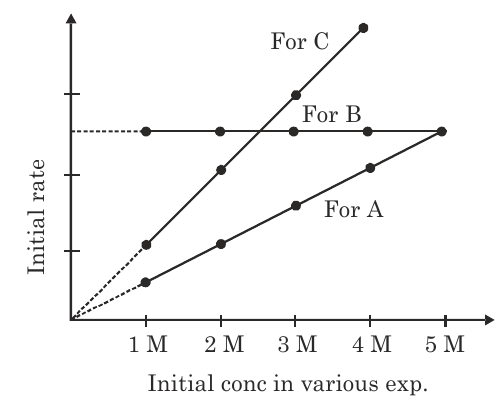
\includegraphics[width=0.7\linewidth]{Score-II - Test 04 (07 May 2021)-img/p1chem_q3_graph.png}
\end{center}

If three reactions:
\[A\longrightarrow\text{Products}\qquad\text{Rate}=K_1[A]^X\]
\[B\longrightarrow\text{Products}\qquad\text{Rate}=K_2[B]^Y\]
\[C\longrightarrow\text{Products}\qquad\text{Rate}=K_3[C]^Z\]
Value of $\left(\dfrac{X+Y}{4Z}\right)$ is?

\textbf{4.}

\begin{center}
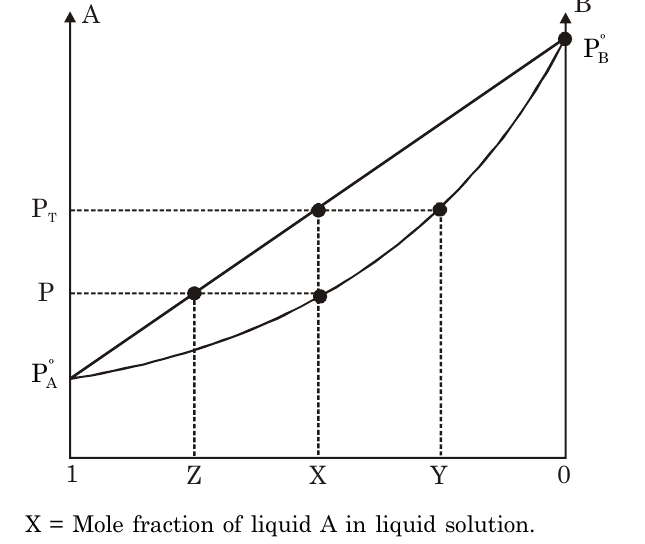
\includegraphics[width=0.6\linewidth]{Score-II - Test 04 (07 May 2021)-img/p1chem_q4_vaporpressure.png}
\end{center}

X $=$ Mole fraction of liquid A in liquid solution.\\
Y $=$ Mole fraction of vapour A in vapour mixture.\\
Z is the graphical mid point between ``1'' \& ``X''.

Find value of $\left(\dfrac{\text{P.Y.}}{100\text{X}}\right)$. [Given: $P_T=450$ mm Hg]

If $P_A^\circ=300$ mm of Hg\\
$P_B^\circ=700$ mm of Hg

\textbf{5.} For an ideal gas sample (fixed amount taken in fixed volume container) collision frequency (Z) \& mean free path ($\lambda$).\\
(i) Both Z \& $\lambda$ changes with change in T.\\
(ii) Z changes with change in T.\\
(iii) $\lambda$ changes with change in T.\\
(iv) Both are independent of temperature T.\\
(v) Heavier gas (more molecular weight) exibits higher Z compared to lighter gas. (if collision diameter of heavier gas is more)\\
(vi) Heavier gas exibits more $\lambda$ compared to lighter gas.\\
(vii) Molecular weight of gas does not have any effect of value of $\lambda$.\\
Identify number of correct statements from above?

\textbf{6.} Assuming ideal geometries without any distortions, find value of $\left(\dfrac PQ\right)$ on basis of following information.

\begin{center}
\small
\renewcommand{\arraystretch}{1.3}
\begin{tabular}{@{}p{0.36\linewidth}p{0.23\linewidth}p{0.23\linewidth}@{}}
\textbf{Properties \& Features} & \textbf{OsCl$_x$\-(CO)$_{2x}$} & \textbf{Os(CO)$_{x+3}$}\\
\midrule
Net dipole moment & Non--zero & Zero\\
C--Os--C bond angles $90^\circ$ \& $180^\circ$ & Yes & Yes\\
Geometrical isomerism possible & Yes & No\\
Maximum number of atoms in single plane & ``P'' & ``Q''\\
\end{tabular}
\normalsize
\renewcommand{\arraystretch}{1.15}
\end{center}

\textbf{7.} Among the given carbonates / bicarbonates, find the value of $\left(\dfrac{x^z}{y}\right)$

KHCO$_3$, NaHCO$_3$, CaCO$_3$, Ca(HCO$_3$)$_2$, K$_2$CO$_3$ and Mg(HCO$_3$)$_2$\\
no. of compounds almost insoluble in water $=$ x\\
no. of compound which liberate CO$_2$ on reaction with HCl $=$ z\\
no. of compounds that easily undergo thermal decomposition $=$ y

\textbf{8.} Halide of Phosphorus PX$_a$ is found to exist in ionic form in solid state, undergoes complete hydrolysis to give two acids H$_b$PO$_c$ and HX. Salt NaX on reaction with conc H$_2$SO$_4$ liberates gas X$_2$. Elemental form of X$_2$ at room temperature is liquid. Value of $\left(\dfrac{\text{at.wt. of X (in amu)}}{a+2b+3c}\right)$

\sectionhdr{PART-3: MATHEMATICS}
\subsectionhdr{Section-I (i): Single Correct}

\textbf{1.} Which of the following statements is correct:

\begin{qoptions}
\opt{A}{Two non collinear vectors are always linearly dependent}
\opt{B}{Two parallel non zero vectors are always linearly independent}
\opt{C}{Any four vectors in 3-d space are always linearly dependent}
\opt{D}{None of these}
\end{qoptions}

\textbf{2.} The solution of the differential equation $\dfrac{dy}{dx}+x(x+y)=x^3(x+y)^3-1$ is:

(Where c is arbitrary constant)

\begin{qoptions}
\opt{A}{$\dfrac{1}{x+y}=x^2+1+ce^x$}
\opt{B}{$\dfrac{1}{(x+y)^2}=x^2+1+ce^{x^2}$}
\opt{C}{$\dfrac{1}{(x+y)^2}=x+1+ce^x$}
\opt{D}{$\dfrac{1}{x+y}=x+1+ce^{x^2}$}
\end{qoptions}

\textbf{3.} A line with direction cosines proportional to 2, 1, 2 meet the lines $x=y+2=z$ and $x+2=2y=2z$ at P and Q respectively. The distance between P and Q is:

\begin{qoptions}
\opt{A}{2}
\opt{B}{3}
\opt{C}{6}
\opt{D}{8}
\end{qoptions}

\textbf{4.} Let $f''(x)<0\ \forall\, x\in\mathbb{R}$ and $g(x)=f(2-x^2)+f(x^2)$ then set of possible values of x for which g(x) is increasing is:

\begin{qoptions}
\opt{A}{$(-1,0)\cup(1,\infty)$}
\opt{B}{$(-\infty,-1)\cup(1,\infty)$}
\opt{C}{$(-\infty,-1)\cup(0,1)$}
\opt{D}{$(-1,1)$}
\end{qoptions}

\textbf{5.} A biased coin with probability of head as $\dfrac23$ is tossed 4 times. If it is known that both head and tail occur, then probability that head and tail occur alternately, is-

\begin{qoptions}
\opt{A}{$\dfrac78$}
\opt{B}{$\dfrac58$}
\opt{C}{$\dfrac38$}
\opt{D}{$\dfrac18$}
\end{qoptions}

\textbf{6.} If $x^8-(k-1)x^4+5=0$, then least possible integral value of `k' so that equation has maximum number of real roots is:

\begin{qoptions}
\opt{A}{4}
\opt{B}{5}
\opt{C}{6}
\opt{D}{7}
\end{qoptions}

\textbf{7.} Sum of squares of slopes of lines which are common tangents to hyperbolas $\dfrac{x^2}{16}-\dfrac{y^2}{9}=1$ and $\dfrac{x^2}{9}-\dfrac{y^2}{16}=-1$ is

\begin{qoptions}
\opt{A}{1}
\opt{B}{2}
\opt{C}{3}
\opt{D}{4}
\end{qoptions}

\textbf{8.} Total number of rectangles which can be formed using the vertices of 16 sided regular polygon is:

\begin{qoptions}
\opt{A}{15}
\opt{B}{21}
\opt{C}{28}
\opt{D}{45}
\end{qoptions}

\subsectionhdr{Section-I (ii): One or more correct (Paragraph based)}

\textit{Paragraph for Questions 9 and 10}

Let $f:\mathbb{R}\to\mathbb{R}$ and $g:\mathbb{R}\to\mathbb{R}$ such that
\[f(x)=\max\{|x|,|x-1|,|x-2|,\ldots,|x-2018|\}\]
\[g(x)=\min\{|x|,|x-1|,|x-2|,\ldots,|x-2018|\}\ \text{then:}\]

\textbf{9.} The value of $\displaystyle\int_0^{2018}f(x)\,dx$ is:

\begin{qoptions}
\opt{A}{1009}
\opt{B}{(1009)$^2$}
\opt{C}{3027}
\opt{D}{3(1009)$^2$}
\end{qoptions}

\textbf{10.} The value of $\dfrac{\displaystyle\int_0^{2018}f(x)\,dx}{\displaystyle\int_0^{2018}g(x)\,dx}$ is

\begin{qoptions}
\opt{A}{3027}
\opt{B}{1009}
\opt{C}{2018}
\opt{D}{6054}
\end{qoptions}

\textit{Paragraph for Questions 11 and 12}

Any matrix $A=[a_{ij}]_{n\times n}$ is said to be symmetric if $A^T=A\Rightarrow a_{ij}=a_{ji}$. Also, trace of matrix A is the sum of elements of principal diagonal of matrix A.

Let S be the set of all possible symmetric matrices of order 3, formed using four 1's, three 2's and two 0's.

\textbf{11.} Number of elements in set S is-

\begin{qoptions}
\opt{A}{12}
\opt{B}{18}
\opt{C}{30}
\opt{D}{36}
\end{qoptions}

\textbf{12.} Sum of traces of all possible matrices in set S is-

\begin{qoptions}
\opt{A}{72}
\opt{B}{90}
\opt{C}{108}
\opt{D}{149}
\end{qoptions}

\subsectionhdr{Section-II: Numerical Value}

\textbf{1.} The value of limit $\displaystyle\lim_{x\to0^-}\left[\dfrac{(1+x)^{1/x}}{e}\right]$ is: (Where [.] represent greatest integer function)

\textbf{2.} Let $f(x)=x^2+2$ and $g(x)=\sqrt{x-2}$ then minimum distance between the curves of f(x) and g(x) is:

\textbf{3.} The probability that value of $\sin^{-1}(\sin x)+\cos^{-1}(\cos y)$, where x, y $\in\{1,2,3\}$ is an integer is $\dfrac1k$, where k is:

\textbf{4.} A bag contains 3 red, 2 white and 2 black balls. Two balls are drawn at random and none of them is found to be a white ball. The probability that both balls are red is $\dfrac ab$ (where a, b are coprime) then $b-a$ is equal to

\textbf{5.} If system of linear equations $(a-1)x+z=\alpha$, $x+(b-1)y=\beta$ and $y+(c-1)z=\lambda$ (where a, b, c $\in\mathbb{Z}$) does not have a unique solution, then maximum possible value of $|a+b+c|$ is:

\textbf{6.} The value of $12\displaystyle\sum_{r=1}^{\infty}\dfrac{(12r^2+1)}{(64r^6-48r^4+12r^2-1)}$ is:

\textbf{7.} Consider the lines\\
$L_1: 2x-y+5=0$\\
$L_2: x+ky-1=0$\\
$L_3: kx+2y+4=0$\\
If the lines $L_1$, $L_2$ and $L_3$ do not form a triangle then absolute value of sum of all possible values of k is

\textbf{8.} On Argand plane, let A be the total number of integral points inside the region $|z|<4$ and B the total number of integral points satisfying $|z-3i|<4$ and $\dfrac{\pi}{6}<(\arg(z-(3i)))<\dfrac{5\pi}{6}$ then the value of $\dfrac AB$ is:

\sectionhdr{PAPER-2}

\sectionhdr{PART-1: PHYSICS}
\subsectionhdr{Section-I (i): One or more correct}

\textbf{1.} An electron in a hydrogen atom makes a transition $n_1\to n_2$ where $n_1$ and $n_2$ are the principal quantum numbers of the two states. Assume Bohr's model is valid in this case. The frequency of the orbital motion of the electron in the initial state is $1/27^{\text{th}}$ of that in the final state. The possible values of $n_1$ and $n_2$ are:

\begin{qoptions}
\opt{A}{$n_1=6,n_2=3$}
\opt{B}{$n_1=4,n_2=2$}
\opt{C}{$n_1=8,n_2=1$}
\opt{D}{$n_1=3,n_2=1$}
\end{qoptions}

\textbf{2.} The refractive index of space changes with y, whose function is given as
\[\mu(y)=\begin{cases}1 & \text{if } y\le0\\ ky^2 & \text{if } 0\le y\le2y_0\\ \dfrac{\ell}{y^2} & \text{if } 2y_0\le y\le4y_0\end{cases}\]
where k and $\ell$ are positive constant. A light ray is incident at point A as shown in figure. When the ray reaches to point B, it becomes parallel to xz-plane. Choose the wrong statement.

\begin{center}
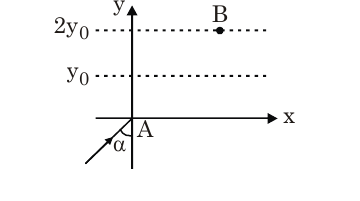
\includegraphics[width=0.4\linewidth]{Score-II - Test 04 (07 May 2021)-img/p2phy_q2_refraction.png}
\end{center}

\begin{qoptions}
\opt{A}{$\alpha$ is independent of k}
\opt{B}{$\alpha$ is independent of $\ell$}
\opt{C}{$\alpha$ is independent of both k and $\ell$}
\opt{D}{$\alpha$ is $90^\circ$}
\end{qoptions}

\textbf{3.} A source emitting sound frequency 1000 Hz moves anticlockwise in the x-y plane along the circle $(x-5)^2+y^2=9$ with a constant speed of 10 m/s where x and y are in meters. A stationary observer is located at the origin. The speed of the sound in air is 330 m/s.

\begin{qoptions}
\opt{A}{X coordinate of the source is 16/5 if frequency heard by the observer is maximum}
\opt{B}{Y coordinate of the source is 12/5 if frequency heard by the observer is maximum}
\opt{C}{X coordinate of the source is 16/5 if frequency heard by the observer is minimum}
\opt{D}{Y coordinate of the source is 36/5 if frequency heard by the observer is minimum}
\end{qoptions}

\textbf{4.} A thin uniform rod of mass 5 kg and length 1 m is held in horizontal position with the help of strings attached to ends of rod. Other ends of strings are held by some external agent. Now end A is pulled down with speed $v_A=3t$ and end B is pulled down with speed $v_B=t$ where t is time in sec. Choose the CORRECT choice(s) at time $t=0$

\begin{center}
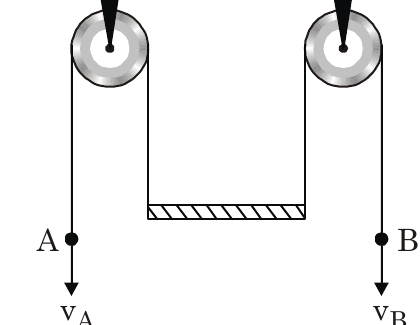
\includegraphics[width=0.5\linewidth]{Score-II - Test 04 (07 May 2021)-img/p2phy_q4_rod.png}
\end{center}

\begin{qoptions}
\opt{A}{Angular acceleration of rod is 2 rad/s$^2$}
\opt{B}{Tension in left string is 185/6 N}
\opt{C}{Acceleration of rod is 1 m/s$^2$}
\opt{D}{Tension in right string is 170/3 N}
\end{qoptions}

\textbf{5.} Two liquid A \& B of specific heat ratio 1:2 are at temperature $2\theta$ and $\theta$ respectively. If they are mixed, then choose CORRECT statement(s): (ignore any heat loss and liquid does not change its state)

\begin{qoptions}
\opt{A}{if equal amount of them are mixed, then temperature of mixture is $\dfrac{3\theta}{2}$}
\opt{B}{if equal amount of them are mixed then temperature of mixture is $\dfrac{4\theta}{3}$}
\opt{C}{if the change of temperature in both the liquid is same then ratio of their masses $\dfrac{m_A}{m_B}=2$}
\opt{D}{if the change of temperature in both the liquid is same then ratio of their masses $\dfrac{m_A}{m_B}=\dfrac32$}
\end{qoptions}

\textbf{6.} Two resistances are measured in Ohm.\\
$R_1=3\Omega\pm1\%$; $\qquad R_2=6\Omega\pm2\%$

\begin{qoptions}
\opt{A}{When they are connected in parallel, the percentage error in equivalent resistance is 4.67\%}
\opt{B}{When they are connected in parallel, the percentage error in equivalent resistance is 0.67\%}
\opt{C}{When they are connected in series, the percentage error in equivalent resistance is 1.66\%}
\opt{D}{When they are connected in series, the percentage error in equivalent resistance is 5\%}
\end{qoptions}

\textbf{7.} A parallel plates capacitor is made of square conducting plates of side a and the separation between plates is d. The capacitor is connected with battery of emf V volt as shown in the figure. There is a dielectric slab of dimension $a\times a\times d$ with dielectric constant k. At $t=0$, dielectric slab is given velocity $v_0$ towards capacitor as shown in the figure. (Neglect the effect of gravity and electrostatic force acting on the dielectric when dielectric is out side of capacitor. Also ignore any type frictional force acting on the dielectric during its motion) let the x be the length of dielectric inside the capacitor at $t=t$ sec. $[\ell_0\gg a]$

\begin{center}
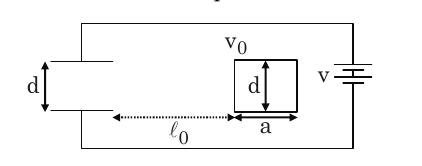
\includegraphics[width=0.5\linewidth]{Score-II - Test 04 (07 May 2021)-img/p2phy_q7_capacitor.png}
\end{center}

\begin{qoptions}
\opt{A}{Motion of dielectric slab is periodic but not simple harmonic motion}
\opt{B}{Motion of dielectric slab is simple harmonic motion}
\opt{C}{At any time, the slope of graph of total energy verses x is twice the slope of graph of potential energy verses x.}
\opt{D}{The value of maximum energy stored in the system is $\dfrac12mv_0^2+\dfrac{\varepsilon_0a^2V^2}{2d}(2k-1)$}
\end{qoptions}

\textbf{8.} A small hole of area 1 cm$^2$ is punched on the side of a cylindrical vessel containing water upto a height $H=10$ m as shown. The torque of normal force about `Centre of the vessel O' immediately after making the hole would be:

Assume that tank does not topple and does not slide and the surface is smooth.

\begin{center}
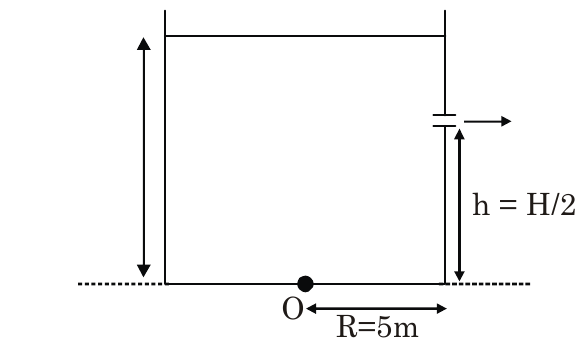
\includegraphics[width=0.4\linewidth]{Score-II - Test 04 (07 May 2021)-img/p2phy_q8_tank.png}
\end{center}

\begin{qoptions}
\opt{A}{10 Nm}
\opt{B}{30 Nm}
\opt{C}{50 Nm}
\opt{D}{Zero}
\end{qoptions}

\subsectionhdr{Section-I (ii): Matching List (Single Correct)}

\textbf{9.} Match the following column:\\
\textbf{List-I} — the coil arrangement shown, \textbf{List-II} — direction of current in coil A at that instant.

\begin{center}
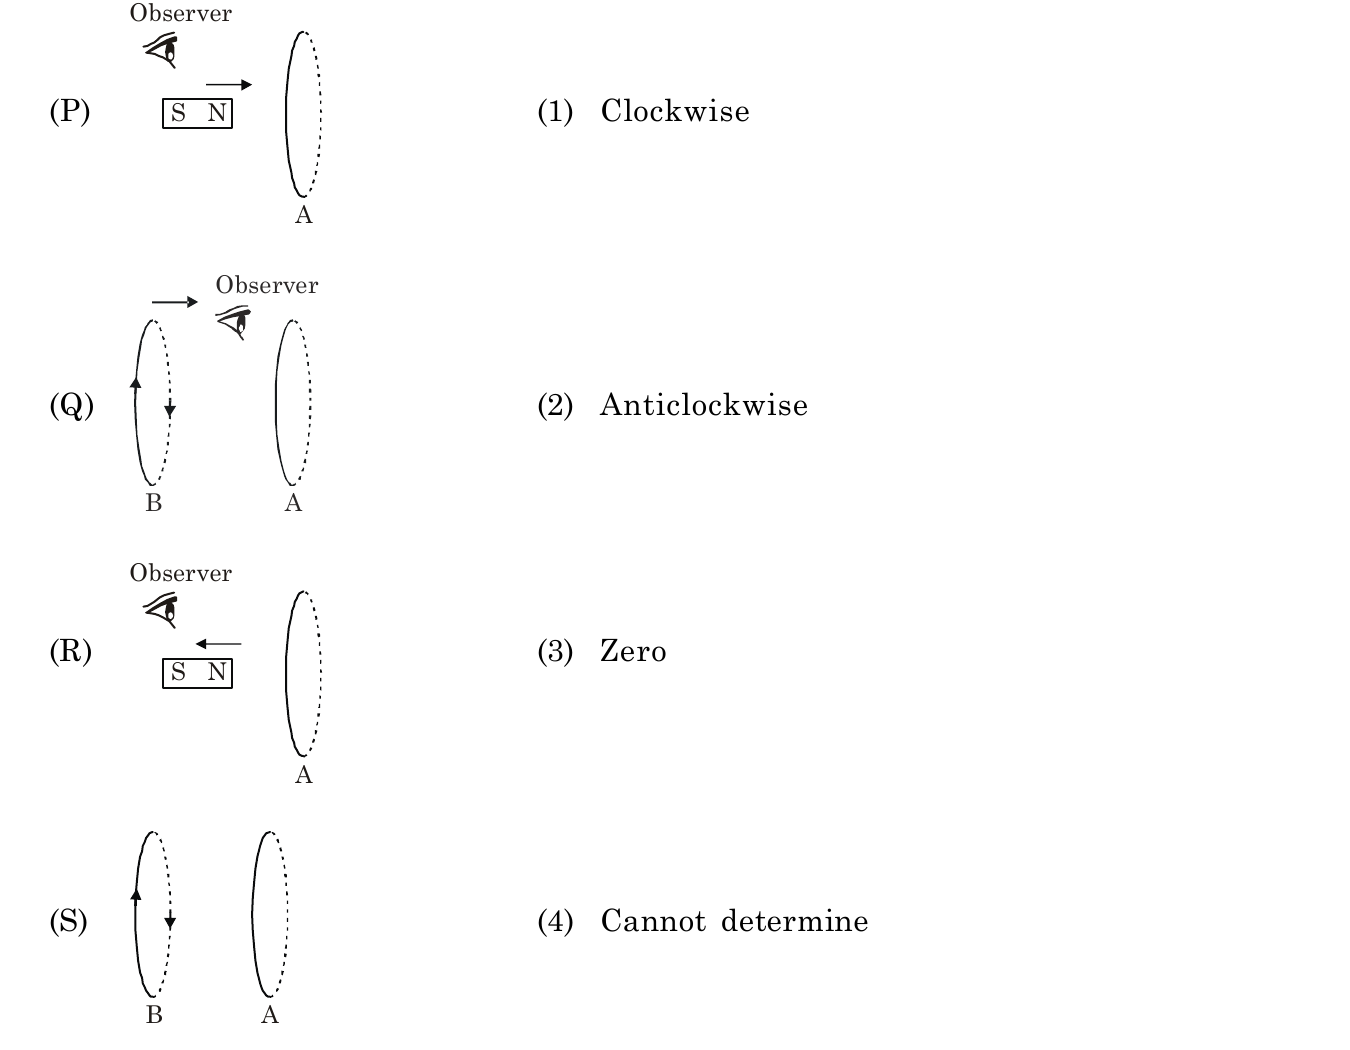
\includegraphics[width=0.85\linewidth]{Score-II - Test 04 (07 May 2021)-img/p2phy_q9_lists.png}
\end{center}

\begin{qoptions}
\opt{A}{P $\to$ 1; Q $\to$ 2; R $\to$ 3; S $\to$ 4}
\opt{B}{P $\to$ 2; Q $\to$ 1; R $\to$ 1; S $\to$ 3}
\opt{C}{P $\to$ 3; Q $\to$ 4; R $\to$ 2; S $\to$ 1}
\opt{D}{P $\to$ 4; Q $\to$ 3; R $\to$ 1; S $\to$ 2}
\end{qoptions}

\textbf{10.} For the situation shown in Fig, match the entries of List-I with entries of List-II.

\begin{center}
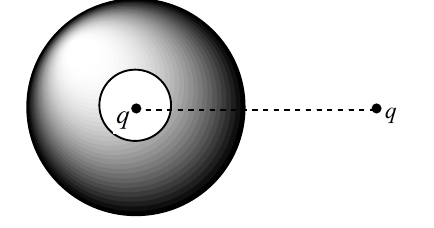
\includegraphics[width=0.45\linewidth]{Score-II - Test 04 (07 May 2021)-img/p2phy_q10_conductor.png}
\end{center}

\begin{center}
\renewcommand{\arraystretch}{1.3}
\begin{tabular}{@{}p{0.45\linewidth}p{0.45\linewidth}@{}}
\textbf{List-I} & \textbf{List-II}\\
(P) If we displace the inside charge and outside charge is not present & (1) distribution of charge on inner surface of conductor is uniform.\\
(Q) If we displace the outside charge keeping the inside charge at center. & (2) distribution of charge on inner surface of conductor is non-uniform.\\
(R) If both the charges are displaced. & (3) distribution of charge on outer surface of conductor is uniform.\\
(S) If outside charge is not present and inside charge is at center, & (4) distribution of charge on outer surface of conductor is non-uniform.\\
\end{tabular}
\renewcommand{\arraystretch}{1.15}
\end{center}

\begin{qoptions}
\opt{A}{P $\to$ 2,3; Q $\to$ 1,4; R $\to$ 2,4; S $\to$ 1,3}
\opt{B}{P $\to$ 1,4; Q $\to$ 2; R $\to$ 3; S $\to$ 4}
\opt{C}{P $\to$ 3; Q $\to$ 1,3; R $\to$ 2; S $\to$ 3}
\opt{D}{P $\to$ 3,4; Q $\to$ 1; R $\to$ 2,4; S $\to$ 1}
\end{qoptions}

\textbf{11.} In the equation X $=$ A sin($\omega t+\pi/4$) match the following:

\begin{center}
\renewcommand{\arraystretch}{1.3}
\begin{tabular}{@{}p{0.45\linewidth}p{0.45\linewidth}@{}}
\textbf{List-I} & \textbf{List-II}\\
(P) Kinetic energy at x $=$ A/2 & (1) Zero\\
(Q) Potential energy at x $=$ A/2 & (2) Maximum\\
(R) Kinetic energy at x $=$ A & (3) $\dfrac14$ times the maximum value\\
(S) Potential energy at x $=$ A & (4) $\dfrac34$ times the maximum value\\
\end{tabular}
\renewcommand{\arraystretch}{1.15}
\end{center}

\begin{qoptions}
\opt{A}{P $\to$ 1; Q $\to$ 2; R $\to$ 3; S $\to$ 4}
\opt{B}{P $\to$ 4; Q $\to$ 3; R $\to$ 1; S $\to$ 2}
\opt{C}{P $\to$ 2; Q $\to$ 4; R $\to$ 2; S $\to$ 3}
\opt{D}{P $\to$ 3; Q $\to$ 1; R $\to$ 4; S $\to$ 1}
\end{qoptions}

\textbf{12.} In radioactivity, number of nuclei of two radioactive substance 1 and 2 are shown in figure.

\begin{center}
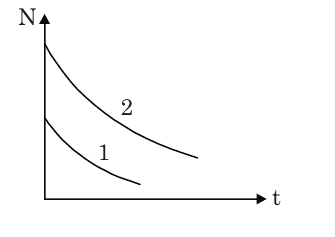
\includegraphics[width=0.4\linewidth]{Score-II - Test 04 (07 May 2021)-img/p2phy_q12_decay.png}
\end{center}

\begin{center}
\renewcommand{\arraystretch}{1.15}
\begin{tabular}{@{}p{0.42\linewidth}p{0.42\linewidth}@{}}
\textbf{List-I} & \textbf{List-II}\\
(P) Initial number of nuclei & (1) 1 \& 2 both are equal\\
(Q) Initial activity of & (2) 1 is more\\
(R) Half life of & (3) 2 is more\\
(S) Decay constant of & (4) Nothing can be said\\
\end{tabular}
\renewcommand{\arraystretch}{1.15}
\end{center}

\begin{qoptions}
\opt{A}{P $\to$ 2; Q $\to$ 1; R $\to$ 4; S $\to$ 2}
\opt{B}{P $\to$ 3; Q $\to$ 2; R $\to$ 4; S $\to$ 1}
\opt{C}{P $\to$ 3; Q $\to$ 1; R $\to$ 3; S $\to$ 2}
\opt{D}{P $\to$ 1; Q $\to$ 3; R $\to$ 2; S $\to$ 3}
\end{qoptions}

\subsectionhdr{Section-II: Numerical Value Type (Up to second decimal place)}

\textit{No question will be asked in section II}

\subsectionhdr{Section-III: Single Digit Integer (0--9)}

\textbf{1.} In an L-C circuit shown in the figure, $C=1$F, $L=4$H. At time $t=0$, charge in the capacitor is 4C and it is decreasing at a rate of $\sqrt5$ C/s. The maximum charge in the capacitor is nC, then value of n will be:

\begin{center}
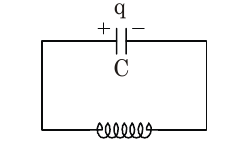
\includegraphics[width=0.28\linewidth]{Score-II - Test 04 (07 May 2021)-img/p2phy_q1_lc.png}
\end{center}

\textbf{2.} Two particles are thrown from same point with same velocity with some time interval between them. Horizontal component of projection velocity is u. The Relative angular velocity of the line joining the two particles when they are at same horizontal level is $n\dfrac gu$, then value of n is

\textbf{3.} Curve shown in the figure is ellipse. If heat energy absorbed by the system in going through this cyclic process is $20n\pi$ joule, then value of `n' is:

\begin{center}
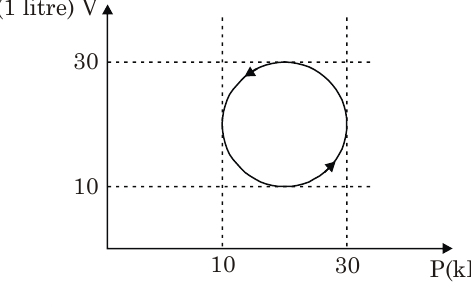
\includegraphics[width=0.5\linewidth]{Score-II - Test 04 (07 May 2021)-img/p2phy_q3_ellipse.png}
\end{center}

\textbf{4.} One end of a light string `L' is tied to a ball and the other end is connected to a fixed point O. The ball is released from rest with string horizontal and just taut. The ball then moves in a vertical circular path as shown in figure; let the velocity of ball at B and C be $\vec V_B$ and $\vec V_C$ respectively. If $|\vec V_C|=2|\vec V_B|$ then the value of $8\sin\theta$ as shown is

\begin{center}
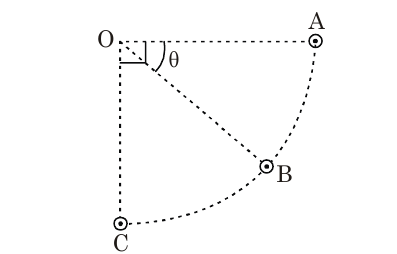
\includegraphics[width=0.42\linewidth]{Score-II - Test 04 (07 May 2021)-img/p2phy_q4_circular.png}
\end{center}

\textbf{5.} A monochromatic light is just able to ionise a hypothetical one electron atom in its ground state, having energy levels defined by $E_n=-\dfrac{17}{n^2}$eV where n is principal quantum number. In an experimental set-up same light is incident on a metal plate and it was found out that electrons have 2eV as maximum kinetic energy. If the work function of metal is 5P eV. Find the value of P.

\textbf{6.} A vertical capillary tube with inside radius 0.25 mm is submerged into water so that the length of its part protruding over the water surface is equal to 25 mm. Surface tension of water is $73\times10^{-3}$ N/m and angle of contact is zero degree for glass and water, acceleration due to gravity is 9.8 m/s$^2$. Then value of 10R approximately (in mm) is (where R is radius of meniscus and h is height of water in capillary tube)

\textbf{7.} A wire of length L is shaped into a circle and then bent in such a way that the two semi-circles are perpendicular. The magnetic moment of the system when current I flows through the system is $\left(\dfrac{\sqrt2\,iL^2}{8\pi}\right)n$, than value of n is

\textbf{8.} If the sound heard by observer, whose equation is given as $y=8\sin10\pi t\cos200\pi t$ at $x=0$, then number of beat frequency heard by observer is 2k. Then the value of k is

\sectionhdr{PART-2: CHEMISTRY}
\subsectionhdr{Section-I (i): One or more correct}

\textbf{1.}

\begin{center}
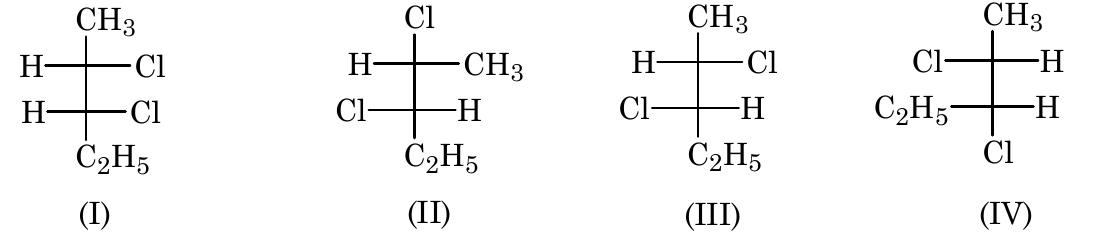
\includegraphics[width=0.95\linewidth]{Score-II - Test 04 (07 May 2021)-img/p2chem_q1_fischer.png}
\end{center}

Which of the following statement are true about these isomers?

\begin{qoptions}
\opt{A}{I and II are a pair of enantiomer}
\opt{B}{III and IV are a pair of enantiomer}
\opt{C}{I and II are a pair of diastereomers}
\opt{D}{I and IV are a pair of diastereomers}
\end{qoptions}

\textbf{2.} Among the given reaction which of the following favours forward reaction.

\begin{center}
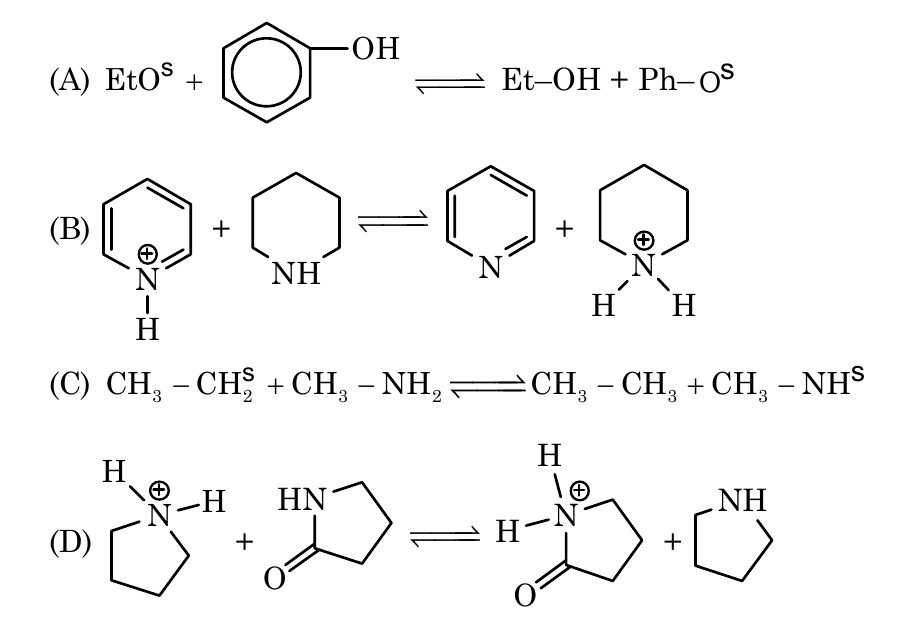
\includegraphics[width=0.9\linewidth]{Score-II - Test 04 (07 May 2021)-img/p2chem_q2_reactions.png}
\end{center}

\textbf{3.} Which of the following statement is correct?

\begin{qoptions}
\opt{A}{p--toludine on treatment with NaNO$_2$ $+$ HCl followed by $\beta$--napthaol in basic medium will give coloured compound.}
\opt{B}{t--BuOH and diethyl ether can be distinguished by Luca's reagent.}
\opt{C}{m-chlorophenol is soluble in aqueous sodium hydroxide}
\opt{D}{Naphthalene and fumaric acid can be seperated by water}
\end{qoptions}

\textbf{4.} Which of the following are correct statements?

\begin{qoptions}
\opt{A}{As$_2$S$_3$ is a negatively charged sol.}
\opt{B}{Brownian movement and Tyndall effect are shown by colloids}
\opt{C}{When liquid is dispersed in liquid, it is called gel.}
\opt{D}{Gold number is a measure of protective power of lyophilic colloid.}
\end{qoptions}

\textbf{5.} As dilution takes place at constant temperature

\begin{qoptions}
\opt{A}{molar conductivity increases}
\opt{B}{conductance increases}
\opt{C}{ionic mobility increases}
\opt{D}{specific conductance increases}
\end{qoptions}

\textbf{6.} CaCO$_3$ decomposed according to the equation $\text{CaCO}_3(s)\rightleftharpoons\text{CaO}(s)+\text{CO}_2(g)$. The equilibrium constant $K_p$ for the reaction is 4 atm. When solid carbon introduced in the vessel a new equilibrium $[\text{CO}_2(g)+\text{C}(s)\rightleftharpoons2\text{CO}(g)]$ is established. The equilibrium constant of this is $2\times10^{-2}$ atm. Then

\begin{qoptions}
\opt{A}{$p_{\text{CO}_2}=4$ atm}
\opt{B}{$p_{\text{CO}}=0.28$ atm}
\opt{C}{At same temperature, if small amount of CaO(s) is added then partial pressure of CO$_2$(g) will decrease.}
\opt{D}{At same temperature, if small amount of CaO(s) is added then partial pressure of CO(g) will remain same.}
\end{qoptions}

\textbf{7.} Among the following, the correct statement(s) is(are)

\begin{qoptions}
\opt{A}{Al(CH$_3$)$_3$ has the three-centre two-electron bonds in its dimeric structure}
\opt{B}{AlCl$_3$ has the three-centre four-electron bonds in its dimeric structure and it is planar}
\opt{C}{BH$_3$ has the three-centre two-electron bonds in its dimeric structure}
\opt{D}{ICl$_3$ is planar in its dimeric structure.}
\end{qoptions}

\textbf{8.} Identify the correct statements.

\begin{qoptions}
\opt{A}{In ClF$_3$ $\angle$FClF bond angle is $90^\circ$.}
\opt{B}{In XeO$_6^{4-}$ all bond length are equal.}
\opt{C}{In NF$_3$ and NH$_3$ bond length N--F $>$ N--H}
\opt{D}{Bond angle in NH$_3$ is more than NF$_3$}
\end{qoptions}

\subsectionhdr{Section-I (ii): Matching List (Single Correct)}

\textbf{9.} Match the list.

\begin{center}
\footnotesize
\renewcommand{\arraystretch}{1.4}
\begin{tabular}{@{}p{0.5\linewidth}p{0.42\linewidth}@{}}
\textbf{List-I} & \textbf{List-II}\\
(P) [Cr(H$_2$O)$_4$Br$_2$]$^+$ & (1) Paramagnetic in nature.\\
(Q) [Cu(NH$_2$CH$_2$CH$_2$NH$_2$)\-(CN)$_2$Cl$_2$]$^{2-}$ & (2) Geometrical isomerism is exhibited.\\
(R) [Pt(OX)$_2$]$^{2-}$ & (3) Central atom in d$^2$sp$^3$ hybridisation\\
(S) [Fe(OH)$_4$]$^-$ & (4) Linkage isomerism is exhibited.\\
& (5) Complex having symmetrical bidented ligand.\\
\end{tabular}
\normalsize
\renewcommand{\arraystretch}{1.15}
\end{center}

\begin{qoptions}
\opt{A}{P $\to$ 1,2,3\quad Q $\to$ 1,2,4,5\quad R $\to$ 5\quad S $\to$ 1}
\opt{B}{P $\to$ 1,2,3,4\quad Q $\to$ 1,2\quad R $\to$ 1,2,3\quad S $\to$ 3,4}
\opt{C}{P $\to$ 2,3,4,5\quad Q $\to$ 1,5\quad R $\to$ 1,2,3\quad S $\to$ 3,4}
\opt{D}{P $\to$ 3\quad Q $\to$ 4,5\quad R $\to$ 1\quad S $\to$ 1,2,3}
\end{qoptions}

\textbf{10.} You are required to match all the metallurgical extractions given in list I with the processes given in list II.

\begin{center}
\renewcommand{\arraystretch}{1.3}
\begin{tabular}{@{}p{0.4\linewidth}p{0.5\linewidth}@{}}
\textbf{List-I (Metallurgical extraction)} & \textbf{List-II (Process involved in metallurgical extraction)}\\
(P) Al$_2$O$_3\cdot2$H$_2$O $\longrightarrow$ Al & (1) Leaching\\
(Q) KCl$\cdot$MgCl$_2\cdot6$H$_2$O $\longrightarrow$ Mg & (2) Self reduction\\
(R) Ag$_2$S $\longrightarrow$ Ag & (3) Electrolytic reduction (molten state)\\
(S) PbS $\longrightarrow$ Pb & (4) Roasting\\
& (5) Displacement method\\
\end{tabular}
\renewcommand{\arraystretch}{1.15}
\end{center}

\begin{qoptions}
\opt{A}{P $\to$ 2,3\quad Q $\to$ 2,4,5\quad R $\to$ 1,2,3\quad S $\to$ 1,4}
\opt{B}{P $\to$ 2,3\quad Q $\to$ 1,3\quad R $\to$ 1,2\quad S $\to$ 3}
\opt{C}{P $\to$ 1,3\quad Q $\to$ 3\quad R $\to$ 1,5\quad S $\to$ 2,4}
\opt{D}{P $\to$ 5\quad Q $\to$ 1,2,3\quad R $\to$ 2\quad S $\to$ 2,3,4}
\end{qoptions}

\textbf{11.} Match the list.

\textbf{List-I}

(P) [1-cyclopentylethanol, structure below] $\xrightarrow{\text{Conc.H}_2\text{SO}_4/\Delta}$

\begin{center}
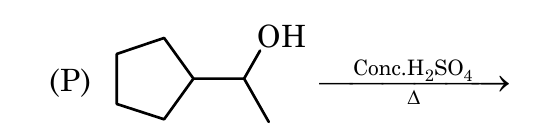
\includegraphics[width=0.35\linewidth]{Score-II - Test 04 (07 May 2021)-img/p2chem_q11_P_structure.png}
\end{center}

(Q) CH$_3$--C(OH)(CH$_3$)--CH$_2$--CH$_3\ \xrightarrow{H^+/\Delta}$

(R) CH$_3$--CH$_2$--CH(Br)--CH$_3\ \xrightarrow{\text{alc.KOH}}$

(S) CH$_3$--CH$_2$--CH(F)--CH$_3\ \xrightarrow{\text{alc.KOH}}$

\textbf{List-II}\\
(1) E$_1$\quad (2) E$_2$\quad (3) Reaction intermediate can rearrange.\quad (4) Saytzeff alkene as the major product\quad (5) Hoffmann alkene as the major product

\begin{qoptions}
\opt{A}{P $\to$ 1,3\quad Q $\to$ 1,4\quad R $\to$ 2,4\quad S $\to$ 2,5}
\opt{B}{P $\to$ 1,3\quad Q $\to$ 1,2\quad R $\to$ 1,2,5\quad S $\to$ 1,2,5}
\opt{C}{P $\to$ 2\quad Q $\to$ 3,4\quad R $\to$ 2,5\quad S $\to$ 1,3,4}
\opt{D}{P $\to$ 1,2,3\quad Q $\to$ 1,3,5\quad R $\to$ 4\quad S $\to$ 1,2,5}
\end{qoptions}

\textbf{12.} Match the thermodynamic processes given list I with the expressions given under list II.

\begin{center}
\renewcommand{\arraystretch}{1.3}
\begin{tabular}{@{}p{0.55\linewidth}p{0.3\linewidth}@{}}
\textbf{List-I} & \textbf{List-II}\\
(P) Melting of ice at 273 K and 1 atm & (1) q $=$ 0\\
(Q) Expansion of 1 mol of an ideal gas into a vacuum under isolated conditions & (2) w $=$ 0\\
(R) Mixing of equal volumes of two ideal gases at constant temperature and pressure in an isolated container & (3) $\Delta S_{\text{sys}}>0$\\
(S) Reversible heating of H$_2$(g) (ideal) at 1 atm from 300 K to 600 K, followed by reversible cooling to 300 K at 1 atm & (4) $\Delta U=0$\\
& (5) $\Delta G=0$\\
\end{tabular}
\renewcommand{\arraystretch}{1.15}
\end{center}

\begin{qoptions}
\opt{A}{P $\to$ 4,5\quad Q $\to$ 3,4\quad R $\to$ 2,3,4\quad S $\to$ 2,4,5}
\opt{B}{P $\to$ 1,4,5\quad Q $\to$ 2,3,4\quad R $\to$ 3,4\quad S $\to$ 1,5}
\opt{C}{P $\to$ 1,2,3,4,5\quad Q $\to$ 1,2,3\quad R $\to$ 3,4\quad S $\to$ 1,5}
\opt{D}{P $\to$ 3,5\quad Q $\to$ 1,2,3,4\quad R $\to$ 1,2,3,4\quad S $\to$ 1,2,4,5}
\end{qoptions}

\subsectionhdr{Section-II: Numerical Value Type (Up to second decimal place)}

\textit{No question will be asked in section II}

\subsectionhdr{Section-III: Single Digit Integer (0--9)}

\textbf{1.} Number of reactions in which aldehyde can be obtained as one of the product.

\begin{center}
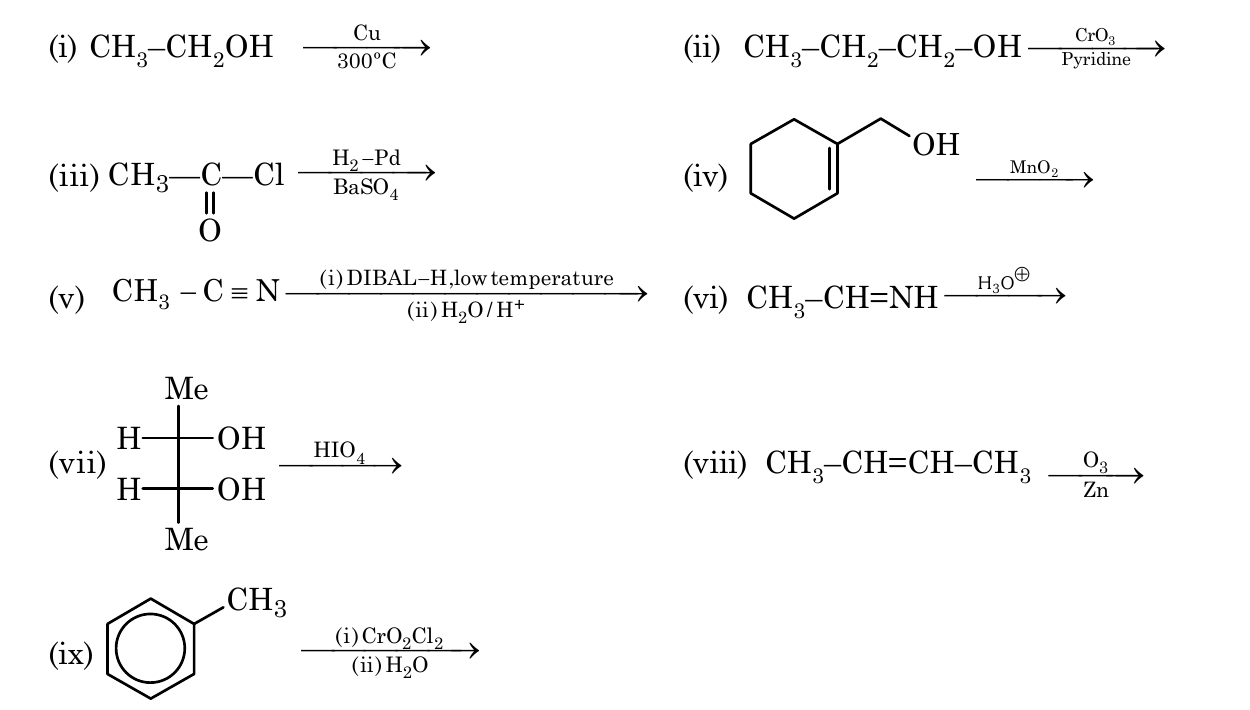
\includegraphics[width=0.85\linewidth]{Score-II - Test 04 (07 May 2021)-img/p2chem_q1_reactions_full.png}
\end{center}

\textbf{2.} How many of the following chemical reactions are correct regarding the product given.

\begin{center}
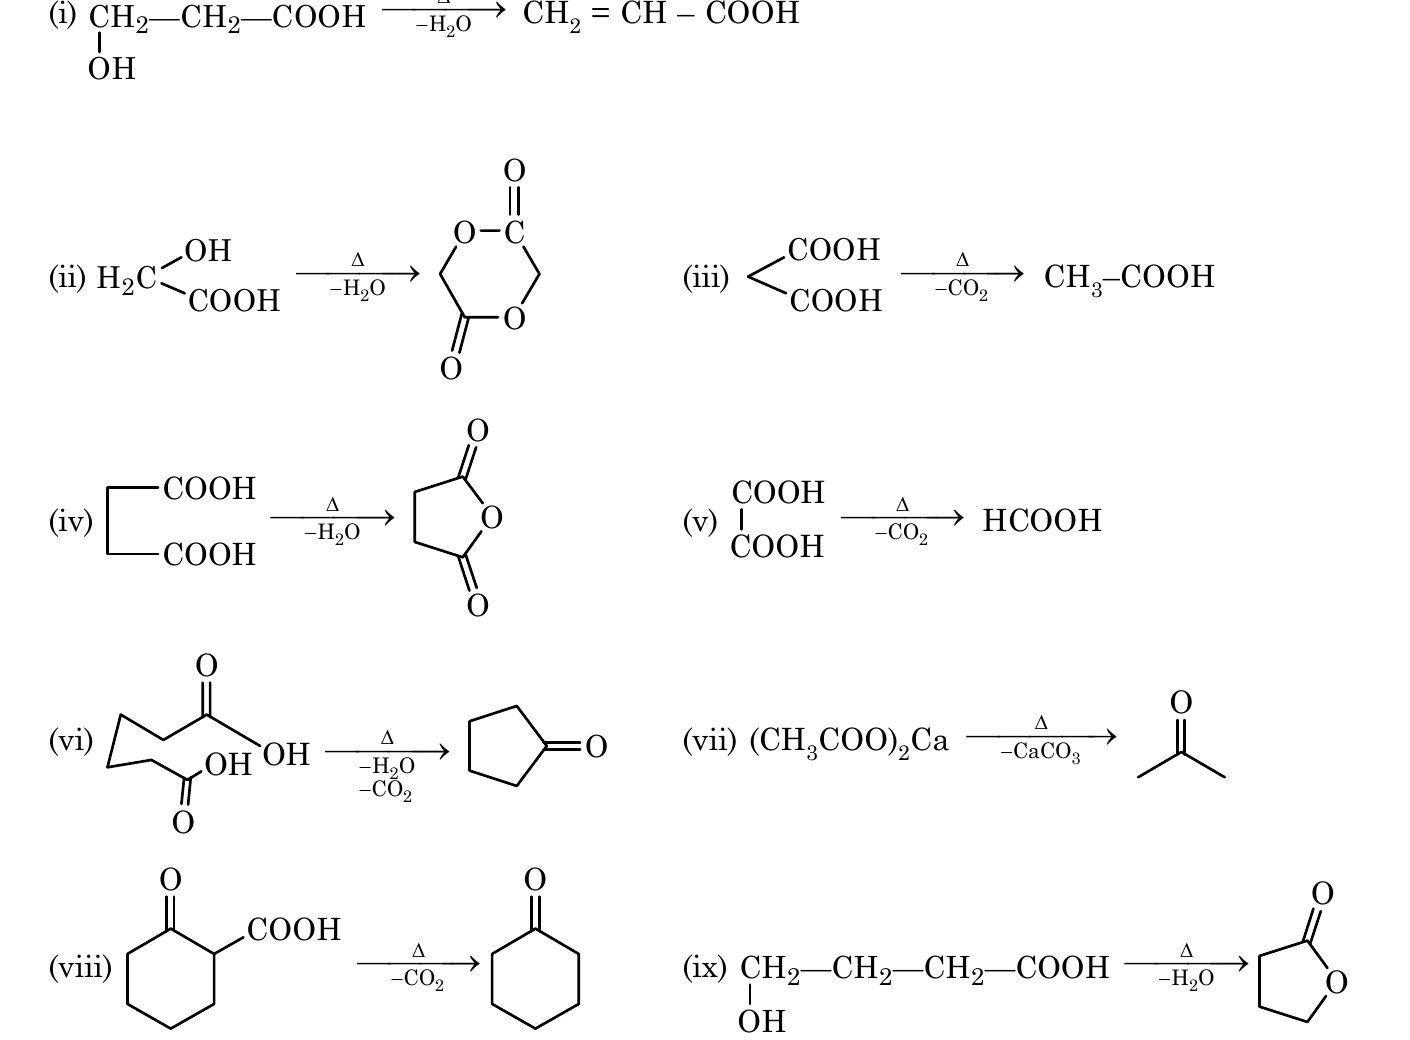
\includegraphics[width=0.95\linewidth]{Score-II - Test 04 (07 May 2021)-img/p2chem_q2_reactions_full.png}
\end{center}

\textbf{3.} How many alcohols belongs to molecular formula C$_7$H$_{14}$O (excluding stereoisomers) and having six or less carbon ring on dehydration with conc. H$_2$SO$_4$ at high temperature give

\begin{center}
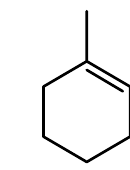
\includegraphics[width=0.18\linewidth]{Score-II - Test 04 (07 May 2021)-img/p2chem_q3_ring.png}
\end{center}

as major product.

\textbf{4.} Green compound (A) $\xrightarrow{\text{Dil.H}_2\text{SO}_4}$ (B)(gas) $+$ C(solution)

C(solution) $\xrightarrow{\text{H}_2\text{S}}$ `D' $\xrightarrow[\text{HNO}_3]{50\%}$ Solution $\xrightarrow{\text{K}_4[\text{Fe(CN)}]_6}$ Chocolate brown ppt.(E)

Solution $\xrightarrow[\text{NH}_4\text{OH}]{\text{excess}}$ Blue complex (F)

Find the total number of unpaired electrons in per molecule of E and F:

\textbf{5.} Select the total number of substance which is/are given below existing as most stable allotrope of corresponding element and having their standard enthalpy of formation zero-\\
(i) Graphite \hspace{1em} (ii) Ozone \hspace{1em} (iii) Black phosphorus \hspace{1em} (iv) Rhombic sulphur\\
(v) White tin \hspace{1em} (vi) Cl$_2$(g) \hspace{1em} (vii) Br$_2$(g)

\textbf{6.} KMnO$_4$ is a good oxidising agent and commonly used to estimate many compounds. 400 ml of KMnO$_4$ solution was divided in two parts. 3/4 part of solution was completely reacted with 200 ml of H$_2$O$_2$ solution and remaining 1/4 part was completely reacted with 200 ml of 50 M H$_2$C$_2$O$_4$ solution, both in acidic medium.

If molarity of KMnO$_4$ is `X' then find the value of $\left(\dfrac{X}{10}\right)$.

\textbf{7.} Out of following how many mixtures are buffers solution\\
(i) NaCN (0.5 mole) \hspace{1em} (ii) NaCN (0.5 moles) $+$ HCN (0.5 moles)\\
(iii) NH$_3$ (1 mole) $+$ NH$_4$Cl (1 mole) \hspace{1em} (iv) CH$_3$COOH (1 mole) $+$ NaOH (0.75 moles)\\
(v) NH$_4$Cl (1 mole) $+$ NaOH (0.75 moles) \hspace{1em} (vi) CH$_3$COONa (0.5 moles) $+$ HCl (0.25 mole)\\
(vii) H$_2$CO$_3$ (1 mole) $+$ NaOH (1.5 moles)

\textbf{8.} How many blood cells of 5ml each having [K$^+$] $=$ 0.1M should burst into 25 ml of blood plasma having [K$^+$] $=$ 0.02 M so as to give final [K$^+$] $=$ 0.06 M

\sectionhdr{PART-3: MATHEMATICS}
\subsectionhdr{Section-I (i): One or more correct}

\textbf{1.} Let f(x) be a non constant twice derivable function defined on R such that $f(2+x)=f(2-x)$ and $f'\left(\dfrac12\right)=0=f'(1)$, then minimum number of roots of the equation $f''(x)=0$ in (0, 4), is

\begin{qoptions}
\opt{A}{4}
\opt{B}{3}
\opt{C}{2}
\opt{D}{5}
\end{qoptions}

\textbf{2.} Let $f(x)=|x^2-5x+6|$, $x\in[0,2.4]$. If M is maximum value of f(x), m is minimum value of f(x), then which of following is/are true

\begin{qoptions}
\opt{A}{Value of M $=$ 6}
\opt{B}{Value of m $=$ 0}
\opt{C}{Value of M $=$ 5}
\opt{D}{M $+$ m $=$ 6}
\end{qoptions}

\textbf{3.} Consider $\displaystyle\int_0^\pi\left(\dfrac{8\sin^2x}{g(x)}-1\right)(g(x))^2\,dx=6\pi$, where g(x) is a continuous positive function in $(0,\pi)$. If the maximum value of g(x) in $(0,\pi)$ is M, then

\begin{qoptions}
\opt{A}{M is a perfect square number}
\opt{B}{M is a prime number}
\opt{C}{M is an even natural number}
\opt{D}{M is an odd prime number}
\end{qoptions}

\textbf{4.} For the expansion of $\left(\sqrt2+3^{1/5}\right)^{10}$, which of the following is/are true

\begin{qoptions}
\opt{A}{Sum of rational terms is 41.}
\opt{B}{There are two rational terms.}
\opt{C}{There are four rational terms.}
\opt{D}{Sum of rational terms is 61.}
\end{qoptions}

\textbf{5.} The circle $|z|=2$ intersects the curve whose equation is $z^2=(\bar z)^2+4i$ in the points A, B, C, D in Argand plane. If $z_1,z_2,z_3,z_4$ represents the affixes of these points, then which of following is/are incorrect.

\begin{qoptions}
\opt{A}{$z_1z_2z_3z_4=1$}
\opt{B}{$\bar z_1+\bar z_2+\bar z_3+\bar z_4=0$}
\opt{C}{$z_1+z_2+z_3+z_4=2$}
\opt{D}{$\arg(z_1)+\arg(z_2)+\arg(z_3)+\arg(z_4)=2k\pi$, where k $=$ 0, 1 or $-1$.}
\end{qoptions}

\textbf{6.} A certain coin lands head with probability P and let Q denotes the probability that when the coin is tossed four times the number of heads obtained is even. Then

\begin{qoptions}
\opt{A}{there is no value of P if Q $=\dfrac14$}
\opt{B}{there is exactly one value of P if Q $=\dfrac34$}
\opt{C}{there are exactly two values of P if Q $=\dfrac35$}
\opt{D}{there are exactly four values of P if Q $=\dfrac45$.}
\end{qoptions}

\textbf{7.} A line meets $\dfrac{x^2}{4a^2}+\dfrac{y^2}{a^2}=1$ at A and B and the parabola $y^2=4ax$ at C and D. The segment AB subtends $90^\circ$ at centre of ellipse. If the locus of point of intersection of tangents to the parabola at C and D is $px^2+qy^2=4a^2$ then the value of p $+$ q is

\begin{qoptions}
\opt{A}{3}
\opt{B}{2}
\opt{C}{5}
\opt{D}{4}
\end{qoptions}

\textbf{8.} For the equation $\cos^{-1}\left(\dfrac{x^2-1}{x^2+1}\right)+\sin^{-1}\left(\dfrac{2x}{x^2+1}\right)+\tan^{-1}\left(\dfrac{2x}{x^2-1}\right)=\dfrac{2\pi}{3}$,

which of the following is/are correct.

\begin{qoptions}
\opt{A}{The number of solution is 2}
\opt{B}{It has at least one irrational solution}
\opt{C}{The sum of solution is positive}
\opt{D}{The sum of solution is negative}
\end{qoptions}

\subsectionhdr{Section-I (ii): Matching List (Single Correct)}

\textbf{9.} Match the following statement in List-I with the values in List-II

\begin{center}
\renewcommand{\arraystretch}{1.4}
\begin{tabular}{@{}p{0.72\linewidth}p{0.12\linewidth}@{}}
\textbf{List-I} & \textbf{List-II}\\
(P) If the range of values of a such that a circle passes through the point of intersection of $y=x^2$ and $x^2-y^2=a^2$ is $(\alpha,\beta)$ then $|\alpha-\beta|$ equals. & (1) 24\\
(Q) The circle $x^2+y^2=1$, cuts the x-axis at P and Q. Another circle with centre at `Q' and variable radius `r' intersects the first circle at R above the x-axis and the line segment PQ at S. If the area of $\triangle$QRS is maximum when $r=\sqrt{\dfrac M3}$, then value of M is & (2) 8\\
(R) Tangents drawn from (4, 4) to the circle $x^2+y^2-2x-2y-7=0$ meet the circle at A and B. If the length of the chord AB is $3\sqrt T$ then value of T is & (3) 2\\
(S) If the distance between centres of two circles of radii 3, 4 units is 25, then length of their transverse common tangent is & (4) 1\\
\end{tabular}
\renewcommand{\arraystretch}{1.15}
\end{center}

\begin{qoptions}
\opt{A}{P $\to$ 1; Q $\to$ 2; R $\to$ 3; S $\to$ 4}
\opt{B}{P $\to$ 4; Q $\to$ 3; R $\to$ 1; S $\to$ 2}
\opt{C}{P $\to$ 4; Q $\to$ 2; R $\to$ 3; S $\to$ 1}
\opt{D}{P $\to$ 3; Q $\to$ 1; R $\to$ 4; S $\to$ 1}
\end{qoptions}


\textbf{10.} Match the following statement in List-I with the values in List-II

\begin{center}
\renewcommand{\arraystretch}{1.5}
\begin{tabular}{@{}p{0.72\linewidth}p{0.12\linewidth}@{}}
\textbf{List-I} & \textbf{List-II}\\
(P) The projection of the vector $(3\hat\imath-4\hat\jmath+2\hat k)$ on the line segment joining the point (2, 3, $-1$) and ($-2$, $-4$, 3) is & (1) $\dfrac12$\\
(Q) Let $\bar\alpha,\bar\beta,\bar\gamma$ are three vectors such that $\bar\alpha+\bar\beta+\bar\gamma=0$ and $|\bar\alpha|=3,|\bar\beta|=5,|\bar\gamma|=7$. If $\theta$ is the angle between $\bar\alpha$ and $\bar\beta$ then value of $\cos\theta$ is & (2) 3\\
(R) If $\bar A=3\hat\imath-\hat\jmath-2\hat k$ and $\bar B=2\hat\imath+3\hat\jmath+\hat k$, then the value of $\left|(\bar A+\bar B)\times(\bar A-\bar B)\right|$ is $2\sqrt P$. Value of $\dfrac{P}{65}$ is & (3) $\dfrac83$\\
(S) If the unit vectors $\bar a,\bar b,\bar c$ are such that $\bar a+\bar b+\bar c=\bar0$ then the value of $\bar a\cdot\bar b+\bar b\cdot\bar c+\bar c\cdot\bar a$ is & (4) $-\dfrac32$\\
\end{tabular}
\renewcommand{\arraystretch}{1.15}
\end{center}

\begin{qoptions}
\opt{A}{P $\to$ 3; Q $\to$ 1; R $\to$ 4; S $\to$ 2}
\opt{B}{P $\to$ 3; Q $\to$ 4; R $\to$ 1; S $\to$ 2}
\opt{C}{P $\to$ 1; Q $\to$ 2; R $\to$ 3; S $\to$ 4}
\opt{D}{P $\to$ 3; Q $\to$ 1; R $\to$ 2; S $\to$ 4}
\end{qoptions}

\textbf{11.} Match the following differential equations in List-I with the general solutions in List-II

\begin{center}
\renewcommand{\arraystretch}{1.5}
\begin{tabular}{@{}p{0.5\linewidth}p{0.35\linewidth}@{}}
\textbf{List-I} & \textbf{List-II}\\
(P) $(xy+2x^2y^2)ydx+(xy-x^2y^2)xdy=0$ & (1) $xy+\ell n\left|\dfrac xy\right|=\dfrac1{xy}+c$\\
(Q) $(x^2y^2+xy+1)ydx+(x^2y^2-xy+1)xdy=0$ & (2) $\ell n\left|\dfrac xy\right|=xy+c$\\
(R) $(x^2+y^2+2x)dx+2ydy=0$ & (3) $x+\ell n(x^2+y^2)=c$\\
(S) $y(1-xy)dx=x(1+xy)dy$ & (4) $2\ell n|x|=\ell n|y|+\dfrac1{xy}+c$\\
\end{tabular}
\renewcommand{\arraystretch}{1.15}
\end{center}

(where `c' is arbitrary constant)

\begin{qoptions}
\opt{A}{P $\to$ 4; Q $\to$ 2; R $\to$ 1; S $\to$ 3}
\opt{B}{P $\to$ 4; Q $\to$ 1; R $\to$ 3; S $\to$ 2}
\opt{C}{P $\to$ 1; Q $\to$ 2; R $\to$ 3; S $\to$ 4}
\opt{D}{P $\to$ 3; Q $\to$ 1; R $\to$ 2; S $\to$ 4}
\end{qoptions}

\textbf{12.} Match the following statement in List-I with the values in List-II

\begin{center}
\renewcommand{\arraystretch}{1.5}
\begin{tabular}{@{}p{0.72\linewidth}p{0.12\linewidth}@{}}
\textbf{List-I} & \textbf{List-II}\\
(P) Let $f:\mathbb{R}\to\mathbb{R}$ be a differentiable function which satisfies $f(x)=\displaystyle\int_0^x|x-f(x)|\,dx\ \forall\, x\in\mathbb{R}$. If $(\alpha,\beta)$ is a point of inflection of f(x), then $\alpha+\beta$ can be & (1) 6\\
(Q) If g(x) is inverse function of f(x) and domain of f(x) is [2, 8] where $f(2)=5$ and $f(8)=2$, then the value of $\displaystyle\int_2^8 f(x)\,dx+\int_5^2 g(y)\,dy$ is & (2) 4\\
(R) $f(x)=|9-x^2|-|x-a|$ then for $a=8$ number of distinct real roots of f(x) & (3) 0\\
(S) $f(x)=|9-x^2|-|x-a|$ then for $a=3$ number of distinct real roots of f(x) & (4) 3\\
\end{tabular}
\renewcommand{\arraystretch}{1.15}
\end{center}

\begin{qoptions}
\opt{A}{P $\to$ 4; Q $\to$ 2; R $\to$ 1; S $\to$ 3}
\opt{B}{P $\to$ 3; Q $\to$ 1; R $\to$ 2; S $\to$ 4}
\opt{C}{P $\to$ 1; Q $\to$ 2; R $\to$ 3; S $\to$ 4}
\opt{D}{P $\to$ 1; Q $\to$ 3; R $\to$ 2; S $\to$ 4}
\end{qoptions}

\subsectionhdr{Section-II: Numerical Value Type (Up to second decimal place)}

\textit{No question will be asked in section II}

\subsectionhdr{Section-III: Single Digit Integer (0--9)}

\textbf{1.} A car is moving at uniform speed towards a tower. It takes 15 minutes for the angle of depression from the top of tower to the car to change from $30^\circ$ to $60^\circ$. The car will reach the base at tower after P minutes. Value of [P] is (Where [.] denotes greatest integer function)

\textbf{2.} The radius of circle passing through the foci of the ellipse $9x^2+16y^2=144$ and having it centre at (0, 3) is

\textbf{3.} If A$_1$ be the A.M. and G$_1$, G$_2$ be two G.Ms between two positive number a and b, then $\dfrac{G_1^3+G_2^3}{G_1G_2A_1}$ is equal to

\textbf{4.} If $x=(2+\sqrt3)^n$, $n\in\mathbb{N}$ then the value of $x-x^2+x[x]$, (Where [.] denotes greatest integer function) is equal to

\textbf{5.} Let B be a skew symmetric matrix of order $3\times3$ with real entries.
Given $I-B$ and $I+B$ are non-singular matrices.
If $A=(I+B)(I-B)^{-1}$ where $\det(A)>0$, then the value of $\det(2A)-\det(\text{adj }A)$ is
[here $\det(P)$ denotes determinant of square matrix P and $\det(\text{adj }P)$ denotes determinant of adjoint of square matrix P respectively]

\textbf{6.} If $\displaystyle\int4(3-2x)^{-2}\left(\dfrac{3-2x}{3+2x}\right)^{1/3}dx=\dfrac3\alpha\left(\dfrac{3+2x}{3-2x}\right)^{\beta/\gamma}+c$ (where c is constant of integration and $\beta,\gamma$ are prime numbers), then value of $(\alpha+\gamma-\beta)$ is

\textbf{7.} If $\displaystyle\lim_{n\to\infty}\dfrac1n\sum_{k=1}^n k\ell n\left(\dfrac{n^2+(k-1)^2}{n^2+k^2}\right)$ exists and is equal to L. The absolute value of [L] is

(Where [.] denotes greatest integer function)

\textbf{8.} The absolute value of the expression $y^3\dfrac{d^2y}{dx^2}$ for the ellipse $3x^2+4y^2=12$ is $\dfrac PQ$ (where P and Q are coprime) then the value of $(P-Q)$ is

\end{document}
